\section{Results}
We gathered a good baseline of data for 80MHz vs 40MHz performance in
both indoor and outdoor environments. Unfortunately, as detailed in
\ref{sec:methodology} we were unable to coherently measure the
performance of different MCS settings. Additionally, we ran out of
time to gather intentionally non-beamformed data for all of the
clients. \todo{discuss what}

All graphs in this section are generated from packet captures
performed by the \texttt{iperf} client unless otherwise noted. Error
bars denote a single standard deviation from the mean.

\subsection{Signal Strength}
We were, however, able to measure beamformed signal strength over
distance and through objects with 80MHz vs 40MHz quite effectively
with both the Intel 7260 and the Macbook. Unfortunately the Surface
was unable to provide radiotap headers during capture, so we have no
information about its recieved signal strength.

\subsubsection{Outdoor Clean Testing}

\begin{figure}[!h]
\centering
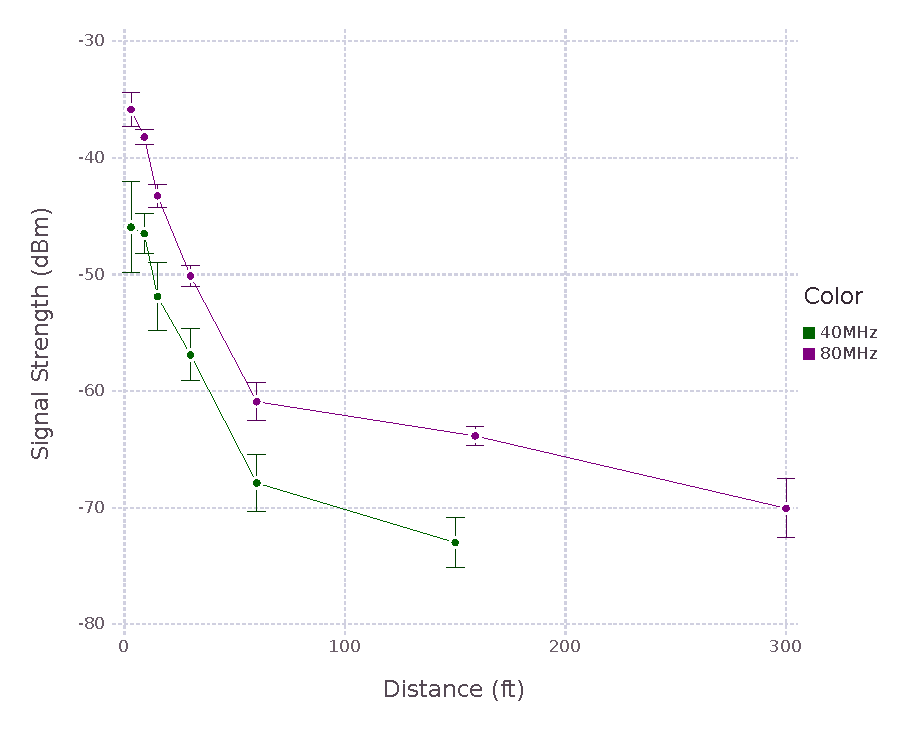
\includegraphics[width=0.5\textwidth]{figures/Intel_Outside_Beamformed}
\caption{Intel Outside Signal Strength Over Distance}
\label{fig:inteloutsidesignal}
\end{figure}

\begin{figure}[!h]
\centering
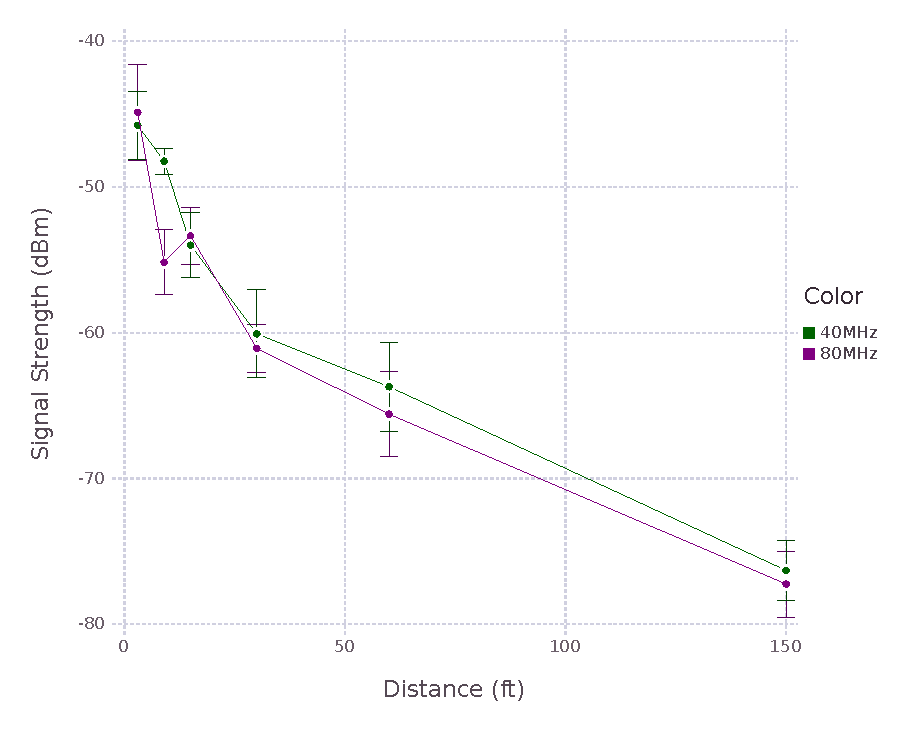
\includegraphics[width=0.5\textwidth]{figures/Mac_Outside_Beamformed}
\caption{Macbook Outside Signal Strength Over Distance}
\label{fig:macoutsidesignal}
\end{figure}


Figure~\ref{fig:inteloutsidesignal} is a perfect example of expected
behavior. As we move away from the WAP, signal strength decreases by
the square of the distance, and since dBm is a logrithmic scale, we
obtain a log-like drop-off! As expected, 80MHz outperforms 40MHz in
all cases, and even manages to maintain a connection over longer
distances.

Somewhat inexplicibly (a common theme in the collected data) the
Macbook (Figure \ref{fig:macoutsidesignal}) had a similar dropoff, but
40MHz consistently outperformed 80MHz! Given the variance shown
however, it is hard to draw any specific conclusions. \todo{this test
  was at the same time as the other...}

\subsubsection{Indoor Noisy Testing}


\begin{figure}[!h]
\centering
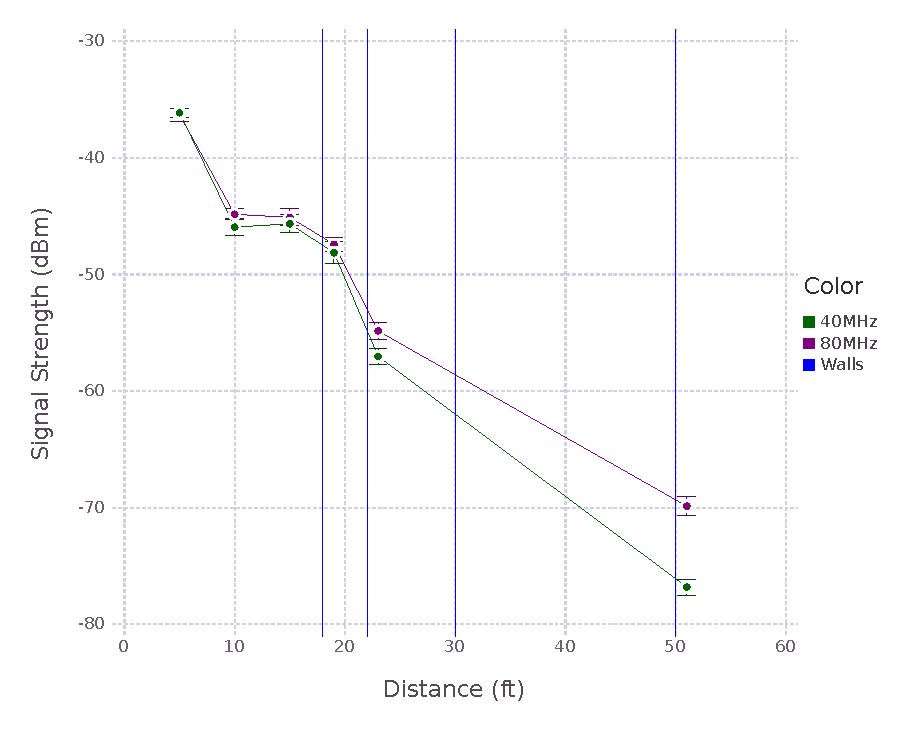
\includegraphics[width=0.5\textwidth]{figures/Intel_Inside_Beamformed}
\caption{Intel Indoor Signal Strength Over Distance}
\label{fig:intelinsidesignal}
\end{figure}

Indoor signal strength does, as expected, drop off significantly
faster than outdoor testing. Figure~\ref{fig:intelinsidesignal} shows
(along with approximate wall locations) the signal strength the Intel
7260 recieved in our office testing. The similar strengths seen betwen
10 and 15 ft is explained by slightly better line-of-sight in the 15ft
case over the 10ft testing location. \todo{need mac graph}

\subsection{Beamforming}
Ideally, we would compare a full non-beamformed conversation to a
beamformed one here. Unfortunately, we were unable to disuade our
client devices from advertising beamformee capabilities, and with
stock firmware the WAP cannot have beamformer capabilities disabled.
This means that while we can compare the recieved signal strength for
beamformed packets vs non-beamformed packets, this is likely to be
biased \emph{against} beamforming looking good. If the WAP decides to
not beamform consistently, it is likely that there is a channel
condition making beamforming tough. \todo{show fig with percentage
  over time?}  Thus, we have Figure~\ref{fig:intelindoorbeamresult}
which would appear to indicate that beamforming \emph{halves} the
incoming power rather than the predicted doubling.

\begin{figure}[h!]
\centering
\begin{tabular}{| c | c |}
\hline
40MHz at 51' & 80MHz at 51'\\ \hline
-2.76 dBm &  -0.31 dBm\\ \hline
\end{tabular}
\caption{Intel 7260 Indoor Beamforming Benefit}
\label{fig:intelindoorbeamresult}
\end{figure}

While still relatively untrustworthy, our outdoor beamforming benefit
measurements are much more in line with expectation.
\todo{need percentage of beamformed packets data}
